\documentclass{beamer}
\usepackage[utf8]{inputenc}
\usepackage{polski}

%\usepackage{utopia} %font utopia imported

\usepackage{multimedia}
\usepackage{graphicx}
%\usepackage{movie15}

\usetheme{Warsaw}
\usecolortheme{default}

%------------------------------------------------------------
%This block of code defines the information to appear in the
%Title page
\title[Mikrofalówka] %optional
{Kuchenka mikrofalowa}

\subtitle{Zasady działania z doświadczeniami}

\author[Lenart, Winiarski] % (optional)
{A.~Lenart\inst{1} \and M.~Winiarski\inst{1}}

\institute[VFU] % (optional)
{
  \inst{1}%
  Wydział Fizyki, Astronomii i Informatyki Stosowanej\\
  Uniwersytet Jagielloński
  %\and
  %\inst{2}%
  %Faculty of Chemistry\\
  %Very Famous University
}

\date[VLC 2014] % (optional)
{Elektryczność i magnetyzm, 27 października 2021}

%\logo{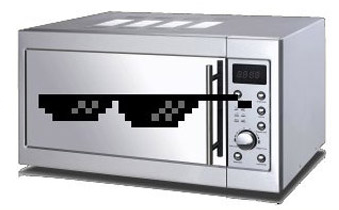
\includegraphics[height=1.5cm]{mikrofaluwka.png}}

%End of title page configuration block
%------------------------------------------------------------



%------------------------------------------------------------
%The next block of commands puts the table of contents at the 
%beginning of each section and highlights the current section:

\AtBeginSection[]
{
  \begin{frame}
    \frametitle{Spis treści}
    \tableofcontents
  \end{frame}
}
%------------------------------------------------------------


\begin{document}

%The next statement creates the title page.
\frame{\titlepage}




\section{Kuchenka mikrofalowa}



%---------------------------------------------------------
%Highlighting text

\subsection{Historia}





\begin{frame}{Historia}

\begin{columns}

\column{0.5\textwidth}
\begin{figure}
    \centering
    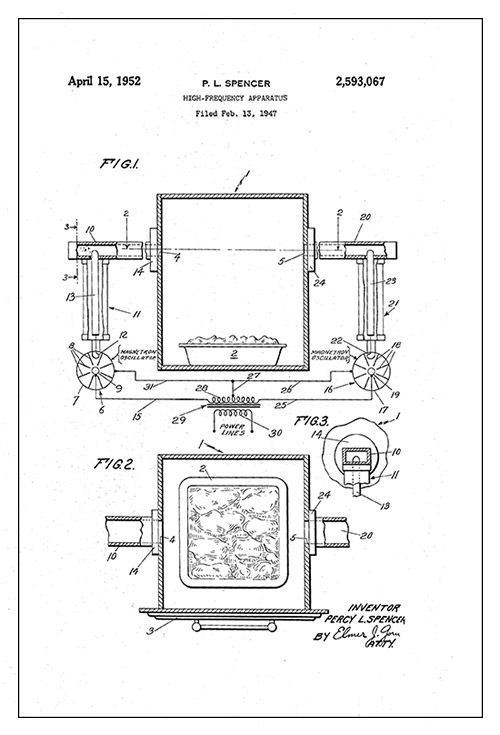
\includegraphics[height=0.79\textheight]{spencer3.jpg}
    %\caption{Rysunek patentowy}
    \label{pat}
\end{figure}\pause

\column{0.5\textwidth}
    \begin{figure}
        \centering
        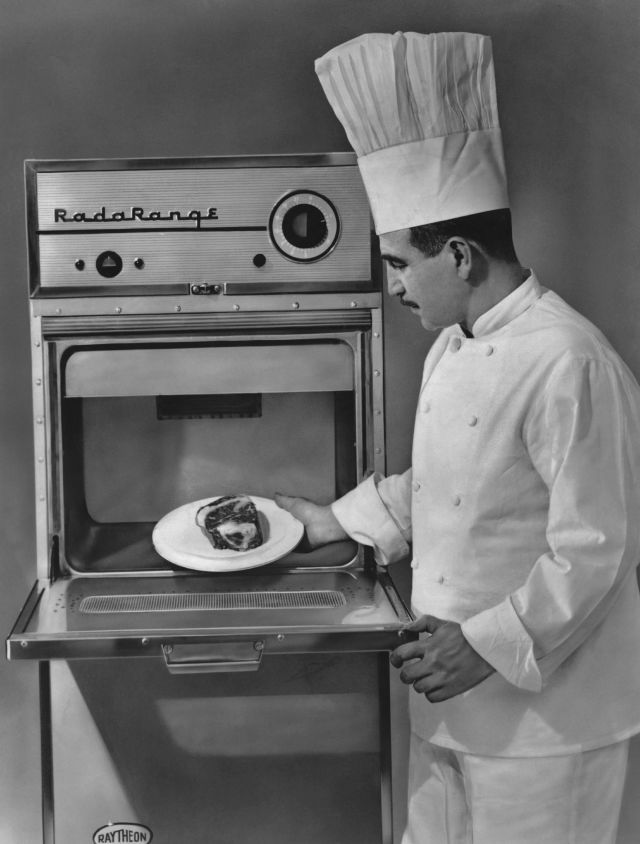
\includegraphics[height=0.75\textheight]{microwave-oven-1.jpg}
        %\caption{Pierwsza kuchenka mikrofalowa}
        \label{rr}
    \end{figure}
    
    \end{columns}
\end{frame}

\subsection{Zasada działania}

\begin{frame}{Schemat}
    \begin{figure}
        \centering
        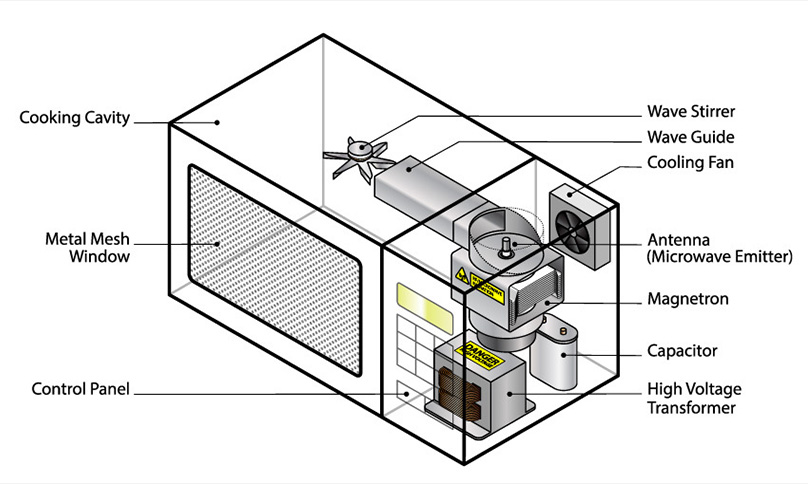
\includegraphics[width=0.8\textwidth]{microwave-diagram.jpg}
        \caption{Schemat mikrofalówki}
        \label{schemat}
    \end{figure}
\end{frame}


\begin{frame}
\frametitle{Magnetron}

\begin{figure}
    %\centering
    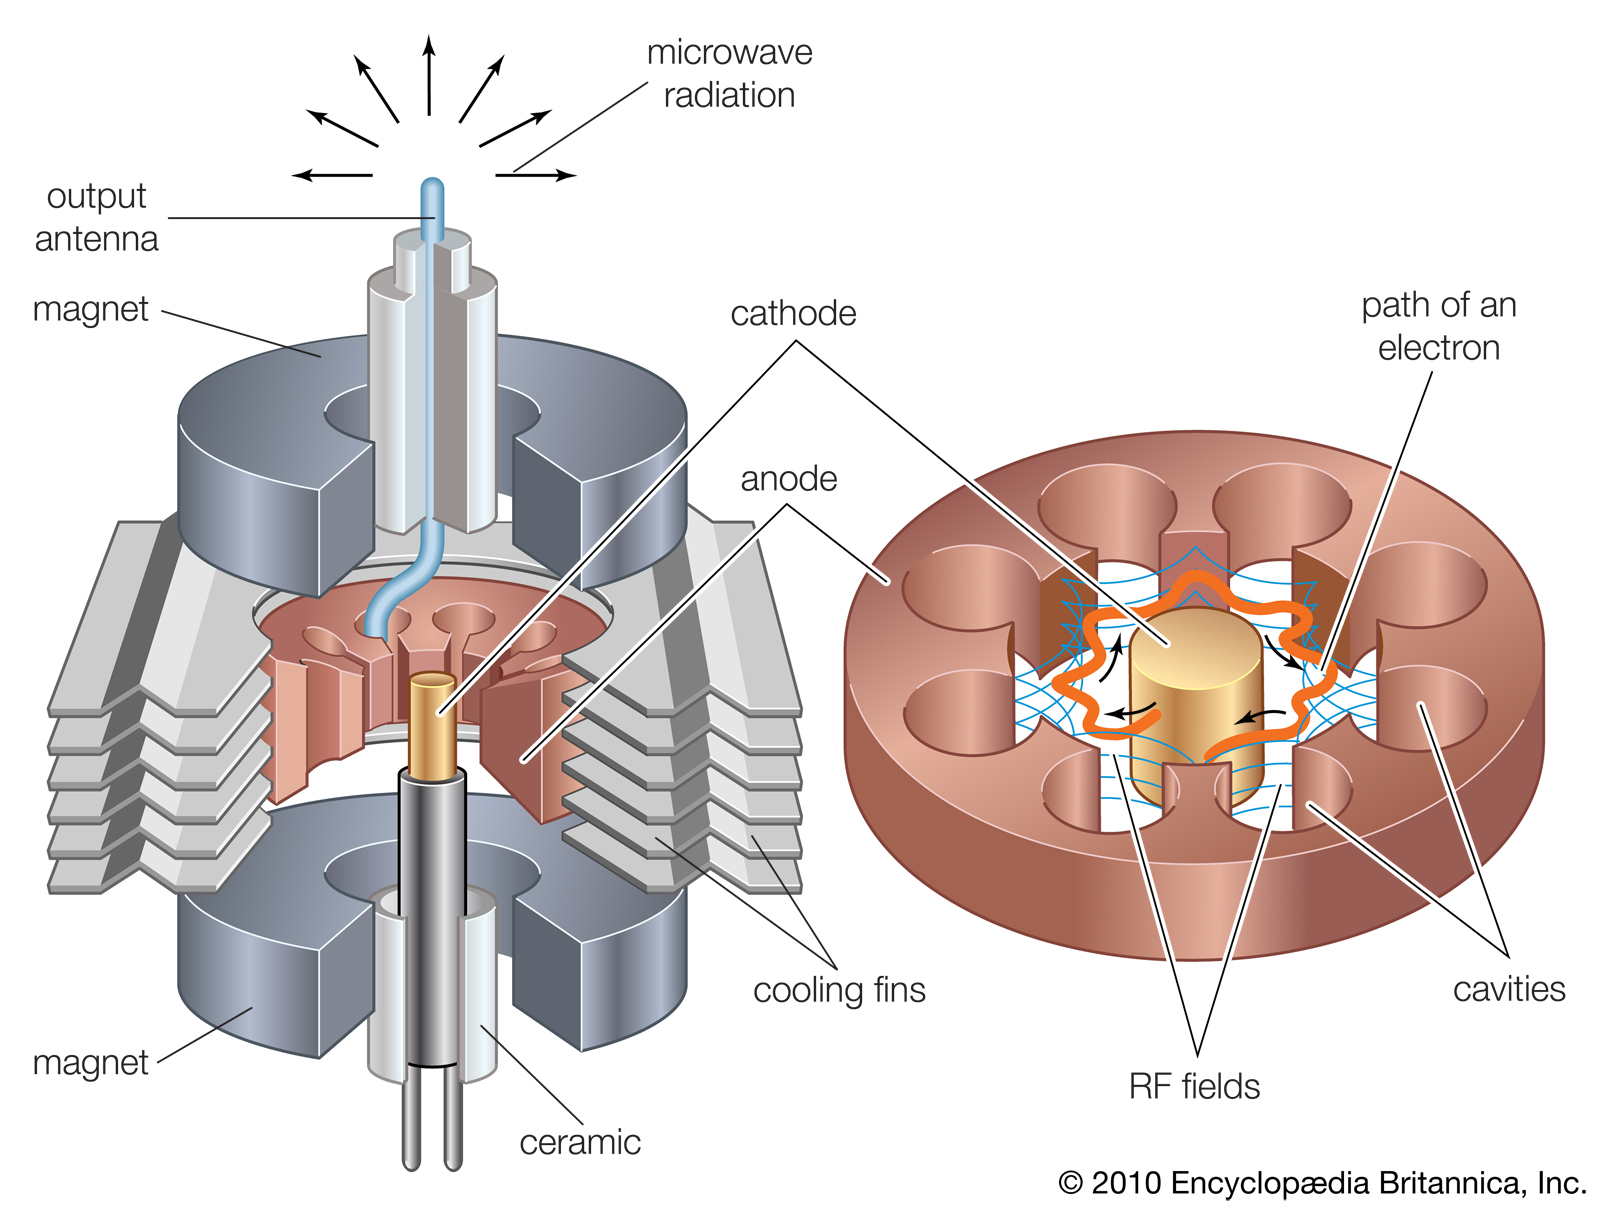
\includegraphics[width=0.8\textwidth]{205-050-C67B86F0.jpg}
    %\caption{Caption}
    \label{megatron}
\end{figure}

\end{frame}
% \begin{frame}
% In this slide, some important text will be
% \alert{highlighted} because it's important.
% Please, don't abuse it.

% \begin{block}{Remark}
% Sample text
% \end{block}

% \begin{alertblock}{Important theorem}
% Sample text in red box
% \end{alertblock}

% \begin{examples}
% Sample text in green box. The title of the block is ``Examples".
% \end{examples}
% \end{frame}
%---------------------------------------------------------

%\subsection{Wykorzystanie}

%---------------------------------------------------------
%Two columns
% \begin{frame}
% \frametitle{Robi jedzonko ciepłe}

% \begin{columns}

% \column{0.5\textheight}
% This is a text in first column.
% $$E^2=m^2c^2+p^2c^4$$
% \begin{itemize}
% \item First item
% \item Second item
% \end{itemize}

% \column{0.5\textheight}
% This text will be in the second column
% and on a second tought this is a nice looking
% layout in some cases.
% \end{columns}
% \end{frame}



\begin{frame}{Częstotliwość fali}

\begin{figure}
    \centering
    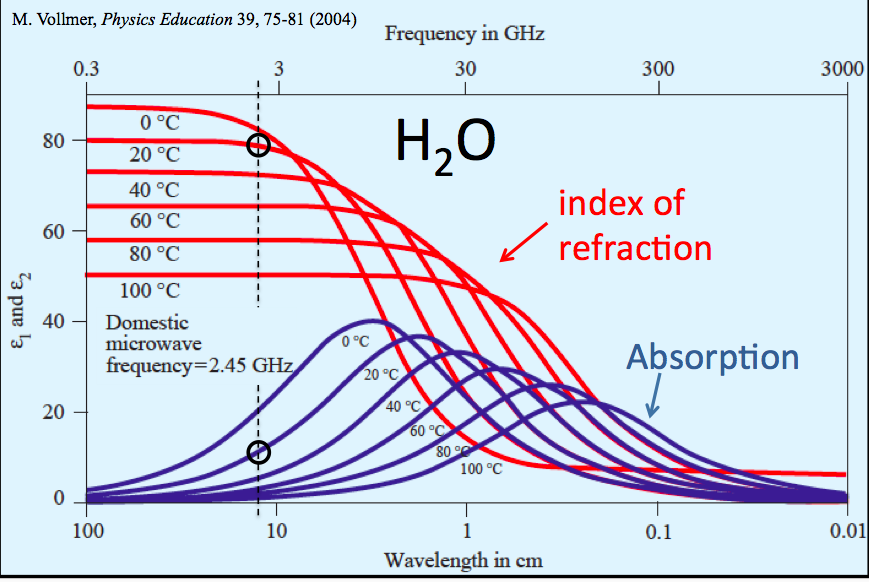
\includegraphics[width=0.8\textwidth]{main-qimg-bd064430fbc98b2fc86cd06d7fc6fd73.png}
    \caption{Zależność pochłaniania i odbijania fali od częstotliwości fali}
    \label{xd}
\end{figure}
    
\end{frame}

\subsection{Wykorzystanie}

\begin{frame}{Wykorzystanie}

\begin{itemize}
    \item Podgrzewanie jedzenia\pause
    \item Szeroko używane w przemyśle do podgrzewania różnych substancji
\end{itemize}

\begin{figure}
    \centering
    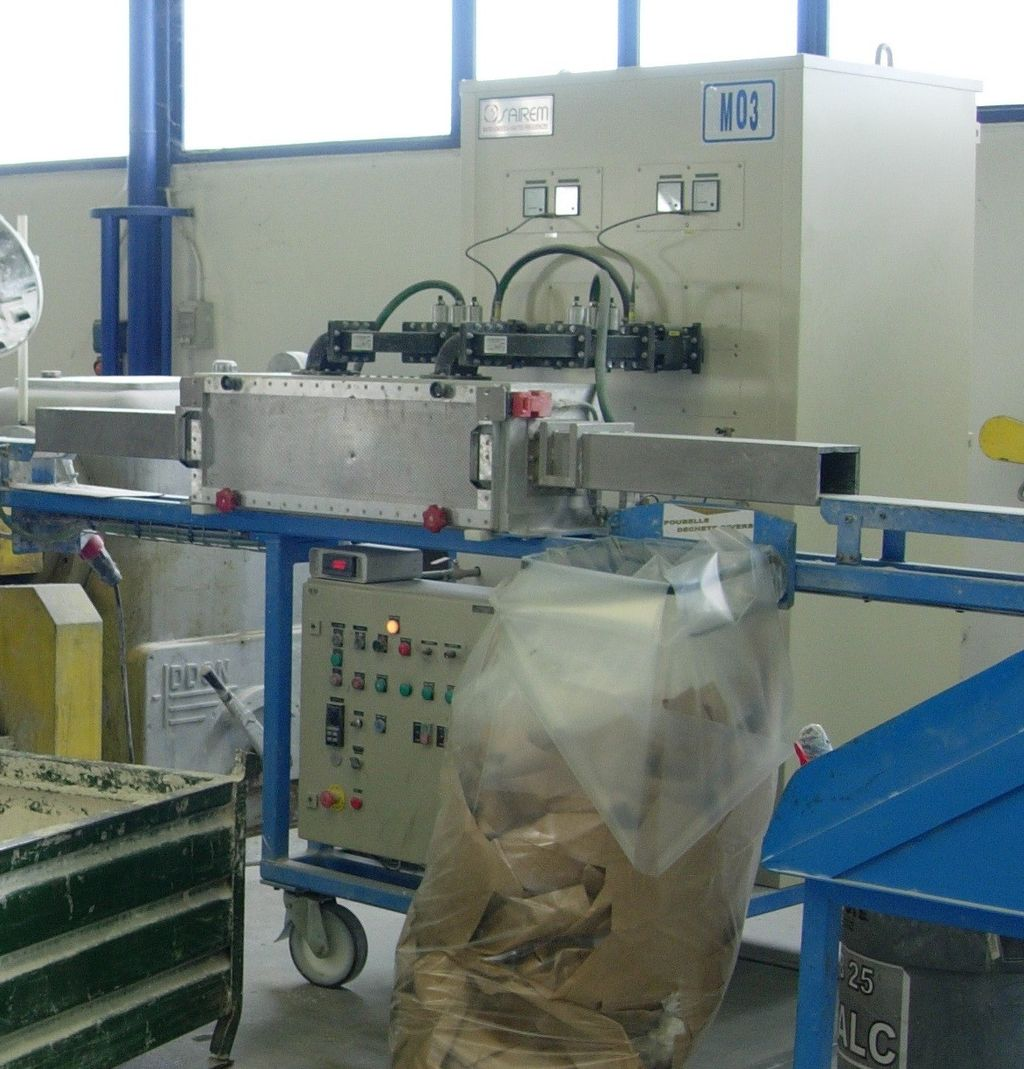
\includegraphics[height=0.55\textheight]{Microwave_tunnel_closeup.jpg}
    \label{fig:my_label}
\end{figure}\pause

\begin{itemize}
    \item 64,6\% gospodarstw domowych w Polsce wyposażonych w kuchenkę mikrofalową
\end{itemize}
    
\end{frame}

\subsection{Demonstracje}

%\subsubsection{Dowód fali w mikrofali}

\begin{frame}{Pomiar prędkości światła}
    \begin{block}{Wzór}
    $$c=\lambda f$$
    \end{block}
\begin{figure}
    \centering
    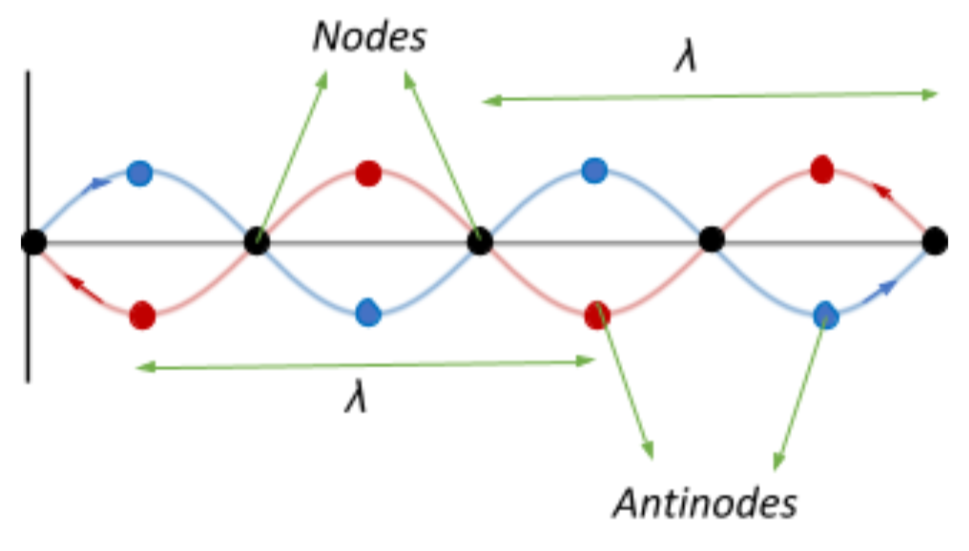
\includegraphics[width=0.5\textwidth]{58d7e603-b9e2-496f-9e49-43f7cce57c094141571019733530534.png}
    \caption{Węzły i strzałki fali stojącej}
    \label{wis}
\end{figure}
\end{frame}

%\subsubsection{Wytworzenie plazmy}
%---------------------------------------------------------
\begin{frame}{Wytworzenie plazmy}
%\movie[width=0.5\textwidth,showcontrols=true]
 %       {% placeholder = text or image
  %          %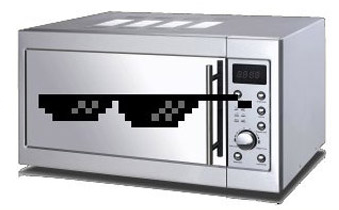
\includegraphics[width=0.4\textwidth]{mikrofaluwka.png}
   %         andrzej
    %    }{videoplayback.mp4}  

\begin{figure}
    \centering
    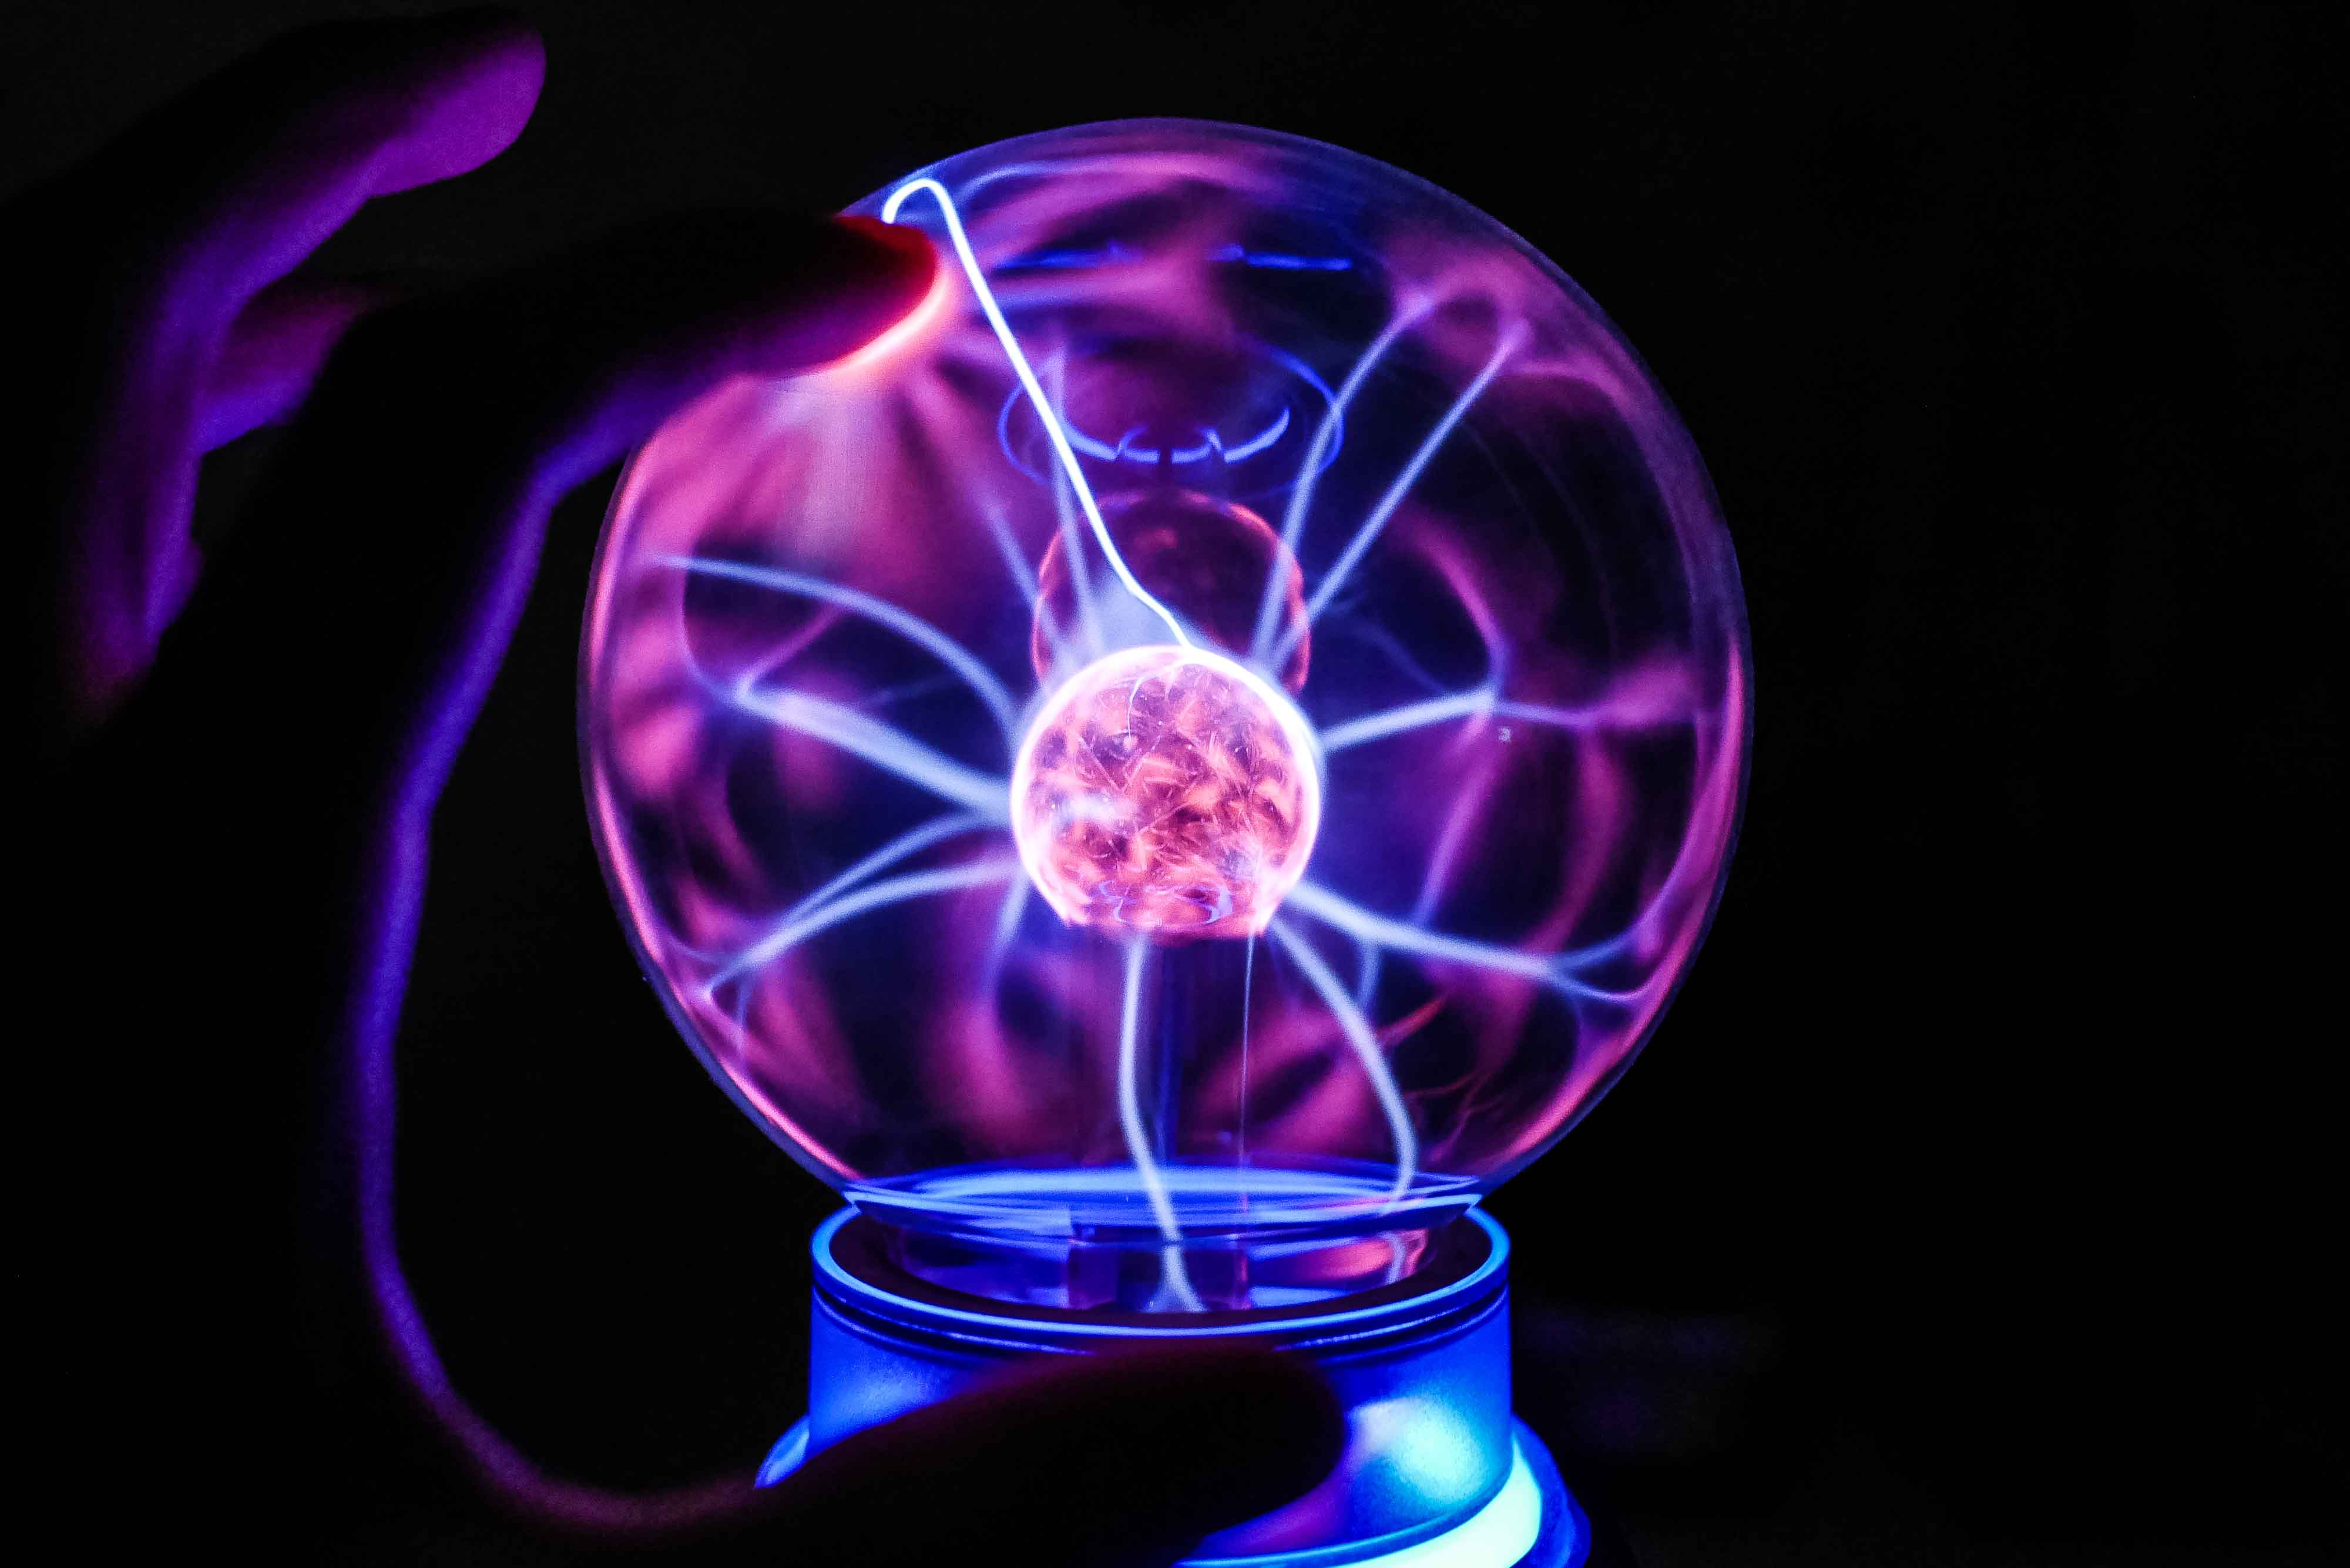
\includegraphics[width=0.8\textwidth]{ how-does-a-plasma-ball-work.jpg}
    %\caption{Plazma}
    \label{fig:my_plasma}
\end{figure}

\end{frame}


\begin{frame}{Bibliografia}
\begin{thebibliography}{}
\bibitem[]{}Vollmer M. 2004. Physics of the microwave oven. Physics Education 39, 74--81. doi:10.1088/0031-9120/39/1/006

\bibitem[Barnes et al.(2021)]{2021AmJPh..89..372B} Barnes, B.~K. and 12 colleagues 2021.\ Plasma generation by household microwave oven for surface modification and other emerging applications.\ American Journal of Physics 89, 372–382. doi:10.1119/10.0002706 %icarus

\bibitem[]{} Główny Urząd Statystyczny 2021. Sytuacja gospodarstw domowych w 2020 r. w świetle wyników badania budżetów gospodarstw domowych.



\end{thebibliography}
\end{frame}

 


\end{document}